\section{Groups, first encounter}
\setcounter{subsection}{0}

\subsection{Definition of group}

% Problem 1.1
\begin{problem}
\end{problem}

\begin{solution}
	Suppose $\C$ is a (non-empty) groupoid. Let $*$ be an object of $\C$. Let $G = \Aut(*)$, we will now prove that $(G, \circ)$ (where $\circ$ is the operation of composition of morphisms in $\C$) is a group. $\circ$ is associative because $\C$ is a category. Let $e_G = 1_*$ and suppose $g \in G$ be any element of $G$. Then $g \circ e_G = g \circ 1_* = g = 1_* \circ g = e_G \circ g$ (again by the definition of a category). Also, since $g \in \Aut(*)$, it is an isomorphism and thus it has a (two-sided) inverse $g^{-1}$. Therefore $(G, \circ)$ is in fact a group.
	
	Now suppose $(G, \bullet)$ is a group. Define $\C$ to be a category with a single object, $*$. We shall define for every $g \in G$ a morphism in $\C$, $g: * \to *$. We identify the identity morphism $1_*$ with $e_G$. The composition will be equal to the operation $\bullet$, as $\bullet: G \times G \to G$ which is equal by our definition to $\bullet: \Hom_{\C}(*,*) \times \Hom_{\C}(*,*) \to \Hom_{\C}(*,*)$. The required properties of morphisms follow from the properties of a group.
	
	Now, suppose $f \in \Hom_{\C}(*,*)$ is a morphism. Then $f \in G$ and there must exist $f^{-1} \in G$, as $G$ is a group. But then $f^{-1} \in \Hom_{\C}(*,*)$, and by the definition of composition $ff^{-1} \equiv f \bullet f^{-1} = e_G \equiv 1_*$. Thus any morphism of $\C$ is necessarily an isomorphism and therefore $\C$ is a groupoid.
	
	Thus any group is in fact a group of isomorphisms of a groupoid. Notice however, that there
	is no need for $\C$ to be a groupoid - every group is in fact a group of automorphisms of some object in some category.
\end{solution}

% Problem 1.2
\begin{problem}
\end{problem}

\begin{solution}
	We will consider the standard operations on numbers, $+,\cdot,-, :$. Lets go over the sets one by one:
	\begin{itemize}
		\item Consider the set $\mathbb{N}$. Now, $+$ will not work, as we could not have inverses. The only possible choice for the identity is $0$, but there is no $a \in \mathbb{N}$ such that, for example, $1+a=0$. $\cdot$ also cannot work, as $0 \cdot 1 = 0 \cdot 2$, but $1 \neq 2$, so cancellation would not work. We cannot use $-$ either, for the same reason as $+$. $:$ also would not work, as we cannot divide by $0$. There are no simple modifications we could do to make those operations work, but as we shall see, we can only consider certain subsets of $\mathbb{N}$ that make $+$ and $\cdot$ work.
		\item Consider $\mathbb{Z}$. $+$ will work, with identity equal to 0. The inverse to any number $z$ will simply be $-z$. $\cdot$ won't work, again by cancellation with $0$. If we considered $\mathbb{Z}$ without $0$, the problem would be the inverses, as for example $2$ does not have an inverse, as for any $a \in \mathbb{Z}$ we have $2 \cdot a \neq 1$ (we either get a greater number, or smaller). $-$ will work similarly to $+$ (being the inverse operation in a sense) and again $:$ won't work.
		\item Consider $\mathbb{Q}$. $+$ will work similarly as for $\mathbb{Z}$. $\cdot$ will only work if we take out $0$ (again because of cancellation). The inverses exist as for $\frac{a}{b}$ we have $\frac{b}{a}$ such that $\frac{a}{b}\cdot\frac{b}{a}=1$. In this case, both $-$ and $:$ work.
		\item Consider $\mathbb{R}$. For this set, all operations will work (taking out $0$, again, for $\cdot$ and $:$). The situation is the same for $\mathbb{C}$. \qedhere
	\end{itemize}
\end{solution}

% Problem 1.3
\begin{problem}
\end{problem}

\begin{solution}
	Consider a group $G$, and $g, h \in G$. Now, $(gh)(h^{-1}g^{-1})=g((hh^{-1})g^{-1})=g(e_Gg^{-1})=gg^{-1}=e_G$. But then $h^{-1}g^{-1}$ is in fact an inverse of $gh$ and since the inverse is unique by Proposition II.1.7, it follows that $(gh)^{-1} = h^{-1}g^{-1}$.
\end{solution}

% Problem 1.4
\begin{problem}
\end{problem}

\begin{solution}
	Consider a group $G$, and $g, h \in G$. Now, since for any $a \in G$, $a^2 = e$, it follows that $g = g^{-1}$ and $h = h^{-1}$ (by Proposition II.1.7). Consider $gh$. We must have $gh = (gh)^{-1} = h^{-1}g^{-1}$ (by Problem II.1.3), but then $gh = hg$, as $h^{-1} = h$ and $g^{-1} = g$. Therefore $G$ is a commutative group.
\end{solution}

% Problem 1.5
\begin{problem}
\end{problem}

\begin{solution}
	Let $(G, \bullet)$ be a group. Consider its multiplication table. Suppose a row, for example the one for some $a \in G$, contains another $b \in G$ twice. But that would mean that there are $c, d \in G$ with $c \neq d$ such that $a \bullet c = b = a \bullet d$, but then by cancellation $c = d$, a contradiction. Similarly for columns.
\end{solution}

% Problem 1.6
\begin{problem}
\end{problem}

\begin{solution}
	The only group with a single element contains just the identity, and thus necessarily $e \cdot e = e$, therefore there is a single multiplication table.
	
	A group with two elements, $a,b$, must contain an identity, thus one row and one column of the multiplication table is given. If $a$ is the identity, the only place that is not clear is $b \cdot b$. But because it is a group, it must follow that $b \cdot b = e$, as otherwise $b$ would not have an inverse (as $a \cdot b = b \cdot a = b \neq a$).
	
	Again, for a group with three elements, one must be the identity. Lets mark the elements $e, a, b$. One row and one column of the multiplication table are again given (the one for $e$). Now, the only choice for $a \cdot b = e$, as if $a \cdot b = a = a \cdot e$, then by cancellation $a = e$, a contradiction. Then it must also be that $a \cdot a = b$ and $b \cdot b = a$, by Problem II.1.5.
	
	Now, consider a group with four elements. We have to decide three rows and three columns. Now for $a \cdot b$ there are two options, $e$ and $c$. $a \cdot b \neq a$ nor $a \cdot b \neq b$ as that would lead to a contradiction by the cancellation law of groups. If $a \cdot b = e$, then we also have $b \cdot a = e$, $a \cdot c = b$ (only $b$ and $c$ are possible but the column contains $c$ already) and thus $a \cdot a = c$. We then have $c \cdot c = e$, thus $b \cdot c = a$, and the other fields follow automatically from Problem II.1.5. automatically (the choice for $a \cdot b$ is in bold):
	
	\begin{center}
		\begin{tabular}{c||c|c|c|c}
			$\cdot$ & $e$ & $a$ & $b$ & $c$ \\
			\hline\hline
			$e$ & $e$ & $a$ & $b$ & $c$ \\ 
			\hline
			$a$ & $a$ & $c$ & $\boldsymbol{e}$ & $b$ \\ 
			\hline
			$b$ & $b$ & $e$ & $c$ & $a$ \\ 
			\hline
			$c$ & $c$ & $b$ & $a$ & $e$ \\ 
		\end{tabular}
	\end{center}

	In case $a \cdot b = c$, we get the following table:
	
	\begin{center}
		\begin{tabular}{c||c|c|c|c}
			$\cdot$ & $e$ & $a$ & $b$ & $c$ \\
			\hline\hline
			$e$ & $e$ & $a$ & $b$ & $c$ \\ 
			\hline
			$a$ & $a$ & $e$ & $\boldsymbol{c}$ & $b$ \\ 
			\hline
			$b$ & $b$ & $c$ & $e$ & $a$ \\ 
			\hline
			$c$ & $c$ & $b$ & $a$ & $e$ \\ 
		\end{tabular}
	\end{center}
		
	In all cases, the groups are commutative, thus all groups with $\leq 4$ elements are necessarily commutative.
\end{solution}

% Problem 1.7
\begin{problem}
\end{problem}

\begin{solution}
	Let $G$ be a group and $g \in G$ an element of finite order, and let $N \in \mathbb{Z}$. Now, suppose $g^N = e$. Then $\abs{g}$ divides $N$ and thus $N$ is a multiple of $\abs{g}$. Now, suppose $N$ is a multiple of $\abs{g}$. Then $N = a\abs{g}$ for some $a \in \mathbb{Z}$. But then $g^N = g^{a\abs{g}}=(g^{\abs{g}})^a=e^a=e$ and thus $g^N = e$.
\end{solution}

% Problem 1.8
\begin{problem}
\end{problem}

\begin{solution}
	Suppose $G$ is a finite abelian group, with exactly one element $f$ of order 2. Consider the product $\prod_{g \in G} g$. Now, since for every $g \in G$, $g \neq f, g \neq e$, we have $\abs{g} > 2$, and thus $g \neq g^{-1}$ (otherwise $\abs{g} = 2$ or $g = e$) the product must contain $g, g^{-1}$. But since $G$ is abelian, we can reorder the product so that the we take the product of $g$ and $g^{-1}$. But this results in $e$, so $\prod_{g \in G} g = ef = f$, exactly as we wanted to prove.
\end{solution}

% Problem 1.9
\begin{problem}
\end{problem}

\begin{solution}
	Let $G$ be a group of order $n$, and let $m$ be the number of elements $g \in G$ of order exactly $2$. Therefore there are $n - m$ elements of $g \in G$ of order not $2$. One of those elements must be $e_G$. Notice, that if $\abs{g} > 2$, $g \neq g^{-1}$. Thus for every element $g$ there must also be its inverse $g^{-1}$ and thus $n - m - 1$ must be even. And therefore $n - m$ is odd.
	
	It then follows that if $n$ is even, there must be elements of $G$ with order $2$. 
\end{solution}

% Problem 1.10
\begin{problem}
\end{problem}

\begin{solution}
	Suppose $G$ is a group and $g \in G$ is an element with odd order. Consider the element $g^2$. By Proposition II.1.13. we then have $\abs{g^2} = \frac{\abs{g}}{\gcd(2, \abs{g})}$. Now since $\abs{g}$ is odd, necessarily we have $\gcd(2, \abs{g}) = 1$. Thus $\abs{g^2} = \abs{g}$.
\end{solution}

% Problem 1.11
\begin{problem}
\end{problem}

\begin{solution}
	Let $G$ be a group, $a, g \in G$ its elements. Let $\abs{g}=N$. Then $(aga^{-1})^N=ag^Na^{-1}=aea^{-1}=aa^{-1}=e$. Therefore $\abs{aga^{-1}}$ must divide $N$. Suppose $\abs{aga^{-1}}=n \leq N$. Then $(aga^{-1})^n=ag^na^{-1}=e$, but then $ag^n=a$, so $g^n=e$, a contradiction, as $n \leq N$, but $N$ is the smallest number such that $g^N = e$. Thus $\abs{aga^{-1}}=\abs{g}$. 
	
	Now, suppose $h \in G$. By the fact we just proved, $\abs{gh} = \abs{hghh^{-1}} = \abs{hge} = \abs{hg}$.
\end{solution}

% Problem 1.12
\begin{problem}
\end{problem}

\begin{solution}
	We have $g^2 =
	\begin{pmatrix}
		-1 & 0\\
		0 & -1
	\end{pmatrix}$, $g^3 =
	\begin{pmatrix}
		0 & 1\\
		-1 & 0
	\end{pmatrix}$, $g^4 =
	\begin{pmatrix}
		1 & 0\\
		0 & 1
	\end{pmatrix}$. Therefore $\abs{g}=4$.
	
	Now, we have $h^2 =
	\begin{pmatrix}
		-1 & -1\\
		1 & 0
	\end{pmatrix}$, $h^3 =
	\begin{pmatrix}
		1 & 0\\
		0 & 1
	\end{pmatrix}$. Therefore $\abs{h}=3$.
	
	But $gh =
	\begin{pmatrix}
		1 & 1\\
		0 & 1
	\end{pmatrix}$, $(gh)^2 =
	\begin{pmatrix}
		1 & 2\\
		0 & 1
	\end{pmatrix}$, $(gh)^3 =
	\begin{pmatrix}
		1 & 3\\
		0 & 1
	\end{pmatrix}$, and so on, so for $n \geq 1$, $(gh)^n =
	\begin{pmatrix}
		1 & n\\
		0 & 1
	\end{pmatrix}$ and thus never equals the identity matrix, and $\abs{gh}=\infty$.
\end{solution}

% Problem 1.13
\begin{problem}
\end{problem}

\begin{solution}
	An easy example is the group of 4 elements with two elements of order $4$ and one of order $2$ from Exercise II.1.6., which we know is commutative. From the multiplication table we can see $\abs{a} = \abs{b} = 4$. But $ab = e$, and therefore $\abs{ab} = 1 \neq \lcm(4, 4)$.
\end{solution}

% Problem 1.14
\begin{problem}
\end{problem}

\begin{solution}
	Let $G$ be a group and $g,h \in G$ elements that commute, so that $gh = hg$. Suppose that $\gcd(\abs{g},\abs{h})=1$. Let $\abs{gh}=N$. Note that by Proposition II.1.14 we have that $N$ divides $\lcm(\abs{g},\abs{h})=\frac{\abs{g}\abs{h}}{\gcd(\abs{g}\abs{h}}=\abs{g}\abs{h}$.
	
	Now, $(gh)^N=g^Nh^N=e_G$ (because $g$ and $h$ commute!). But then $e_G=e_G^{\abs{h}}=(gh)^{N \abs{h}}=g^{N\abs{h}}h^{N\abs{h}}=g^{N\abs{h}}$. But then by Proposition II.1.11 it follows that $\abs{g}$ divides $N\abs{h}$. But since $\gcd(\abs{g},\abs{h})=1$, it follows that $\abs{g}$ divides $N$. Similarly we get that $\abs{h}$ divides $N$. But again by $\gcd(\abs{g}\abs{h})=1$, it follows that $\abs{g}\abs{h}$ divides $N$.
	
	But then $N = \abs{gh} = \abs{g}\abs{h}$. 
\end{solution}

% Problem 1.15
\begin{problem}
\end{problem}

\begin{solution}
	Let $G$ be a commutative group and let $g \in G$ be an element of maximal finite order, that is for any $h \in G$, if $h$ has finite order, then $\abs{h} \leq \abs{g}$. Now, let $h$ be an element of finite order. Suppose that $\abs{h}$ does not divide $\abs{g}$. Then there is a prime number $p$ such that $\abs{g}=p^m r$ and $\abs{h}=p^n s$ for some integers $m, n, r, s$ such that $r$ and $s$ are relatively prime to $p$ and $m < n$ (as if such a prime would not exist, i.e. if $n \leq m$ for all primes in the factorizations of $g$ and $h$, then $h$ would divide $g$). 
	
	Now, $\abs{g^{p^m}}=\frac{\abs{g}}{\gcd(\abs{g},p^m)}=\frac{\abs{g}}{p^m}=r$. $\abs{h^s}=\frac{\abs{h}}{s}=p^n$. Clearly $\gcd(\abs{g^{p^m}},\abs{h^s})=1$ and thus $\abs{g^{p^m}h^s}=\abs{g^{p^m}}\abs{h^s}=p^n r$ (by Exercise II.I.14.). But $p^n r > p^m r = \abs{g}$ (as $n > m$), a contradiction to the assumption that $g$ is an element of maximal finite order.
\end{solution}

\subsection{Examples of groups}

% Problem 2.1
\begin{problem}
\end{problem}

\begin{proof}
	Let $S_n$ be the group of permutations of the set $\set{1,2,\dots,n}$ and let $\sigma,\tau \in S_n$. Associate the $n \times n$ matrices $M_\sigma, M_\tau$ to those permutations as in the text, i.e. for $M_\sigma$ the entry at $(i, (i)\sigma)=1$ for all $i \in \set{1,2,\dots,n}$ and all other entries will be $0$. Consider the matrix $M_\sigma M_\tau$. The entry at $(i,j)$ must be equal to $(i,1)(1,j)+(i,2)(2,j)+\dots+(i,n)(n,j)$ by the definition of matrix multiplication. Now, by the definition of $M_\sigma$ and $M_\tau$, for the entry to equal $1$, there must be a $k$ such that $(i,k)=(k,j)=1$, but that can only happen, again by the definition, if $k = (i)\sigma$ and $j = (k)\tau=((i)\sigma)\tau=(i)\sigma\tau$ (because $S_n$ is a group). Therefore, by the definition of $M_{\sigma\tau}$, $M_{\sigma\tau}=M_\sigma M_\tau$.
\end{proof}

% Problem 2.2
\begin{problem}
\end{problem}

\begin{proof}
	Suppose $S_n$ is the group of permutations of the set $\set{1,2,\dots,n}$. Let $d$ be a positive integer such that $d \leq n$. Consider the permutation 
	\[\sigma =
	\begin{pmatrix}
		1 & 2 & 3 & \dots & d & d + 1 & \dots & n\\
		d & 1 & 2 & \dots & d - 1 & d + 1 & \dots & n
	\end{pmatrix}
	=
	\begin{pmatrix}
	1 & 2 & 3 & \dots & d\\
	d & 1 & 2 & \dots & d - 1
	\end{pmatrix}
	\].
	Clearly, $\sigma^d=e$ and for any $m \leq d$ we have $\sigma^m \neq e$, as $(1)\sigma^m=(d)\sigma^{m-1}=(d-1)\sigma^{m-2}=\dots=d-(m-1)$. Therefore $\sigma$ has order $d$.
\end{proof}

% Problem 2.3
\begin{problem}
\end{problem}

\begin{proof}
	We use the same construction of permutations as we used in Problem II.2.2.
\end{proof}

% Problem 2.4
\begin{problem}
\end{problem}

\begin{proof}
	Label a square as follows:
	\begin{equation*}
	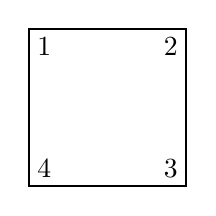
\begin{tikzpicture}
		\node[draw=black, thick,minimum width=2cm,minimum height=2cm] (rect) at (0,0) {};
		\foreach \anc/\n in {south west/4,north west/1,north east/2,south east/3}{
			\node[anchor=\anc] at (rect.\anc) {\n};
		}
	\end{tikzpicture}
	\end{equation*}
	Now, there are four rotations of this square about its center, resulting in the permutations (falling to the shorter notation) $(1\;2\;3\;4), (2\;3\;4\;1), (3\;4\;1\;2), (4\;1\;2\;3)$. There are two reflections about a line passing through the center and one of the vertices (as if the line passes through one vertex, it also passes by the one directly across the center), those result in the permutations $(1\;4\;3\;2)$ and $(3\;2\;1\;4)$. There are also the two reflections about a line passing through the center and a middle of one of the sides, there we get $(2\;1\;4\;3)$ and $(4\;3\;2\;1)$. But that is all the $8$ symmetries of this square, thus we have a homomorphism $D_8 \to S_4$.
\end{proof}

% Problem 2.5
\begin{problem}
\end{problem}

\begin{solution}
	Let $D_{2n}$ be a dihedral group, i.e. the group of symmetries of a regular polygon with $n$ vertices. Let $x$ be a reflection about the center of the polygon and any vertex. Clearly, it must hold that $x^2 = e$, as reflecting about the same line twice returns all the vertices to their original places. Let $y$ be a counterclockwise rotation by $2\pi/n$. Rotating the polygon $n$ times gives us back the original polygon, and thus $y^n=e$.  Now, notice that composing those two symmetries like $xyxy$ gives us back the original polygon, thus $(xy)^2=e$. Manipulating this equation we get $yx=xy^{-1}=xy^{n-1}$ (as $y^{-1}=y^{n-1}$). 
	
	Using these relation we can simplify any product in $D_{2n}$. Suppose $x^{i_1}y^{j_1}x^{i_2}y^{j_2}\dots$ is such a product and without loss of generality suppose $i_k < 2$ and $j_k < n$ for $k \in \mathbb{N}$ (due to the $x^2=e$ and $y^n=e$ relations). Now, we can use the relation $yx = xy^{n-1}$ to move all the $x$ in the product to the right. Thus we can in fact simplify any product in $D_{2n}$ to $x^i y^j$ for $0 \leq i < 2, 0 \leq j < n$.
\end{solution}

% Problem 2.6
\begin{problem}
\end{problem}

\begin{solution}
	For the case $n=1$, we can easily take $g=h$, since $\abs{g}=2$, we have $gg=e$ and thus $\abs{gh}=1$ as needed.
	
	Now suppose $n > 1$. Now consider the group $D_{2n}$. By Problem II.2.5. there are elements $x,y \in D_{2n}$ such that $\abs{x}=2$, $\abs{y}=n$ and $\abs{xy}=2$. Let us define $g = xy$ and $h = x$ (so that $\abs(g)=\abs(h)=2$). We have $gh = xyx = y^{-1}$ and thus $\abs{gh}=\abs{y^{-1}}=\abs{y}=n$.
\end{solution}

% Problem 2.7
\begin{problem}
\end{problem}

\begin{solution}
	By Problem II.2.6. any element of $D_{2n}$ can be written as a product $xy^i$ or $y^i$, $0 \leq i < n$. Now, consider the elements of the form $y^i$, $0 < i < n$. For $y^i$ to commute with $x$, we need to have $x y^i=y^i x$ by definition. But $x y^i = x y y^{i-1} = y^{-i} x$ (as $\abs{xy}=2$). But that means $y^i = y^{-i}=(y^i)^{-1}$ and thus $\abs{y^i}=2$. But by Proposition I.1.13. we know that $\abs{y^i}=\frac{\abs{y}}{\gcd(i, \abs{y}}=\frac{n}{\gcd(i,n)}=2$. So in particular $\gcd(i,n)=\frac{n}{2}$. Since $i < n$, it follows that $i=\frac{n}{2}$.
		
	Now consider elements of the form $xy^i$. If such an element commutes with everything, it has to commute with $x$ in particular. We have $xxy^i=y^i$ and $xy^ix=x^2y^{-i}=y^{-i}$. Now this can only happen for $i = \frac{n}{2}$. Now, it must also commute with $y$. We have $yxy^i=xy^{i-1}$ and $xy^{i}y=xy^{i+1}$. Now, $xy^{i-1}=xy^{i+1}$ would mean $y^{i-1}=y^{i+1}$, which in turn would mean $y^2=e$. But that only happens if $n=2$.
	
	Therefore we have found that there are no elements that commute with everything for groups $D_{2n}$ where $n$ is odd. In the case $n=2$, $y$ and $xy$ commute with everything. In the case $n > 2$, the only such element is $y^{\frac{n}{2}}$, which of course only exists if $n$ is even.
\end{solution}

% Problem 2.8
\begin{problem}
\end{problem}

\begin{solution}
	[not interested]
\end{solution}

% Problem 2.9
\begin{problem}
\end{problem}

\begin{solution}
	Let $n\in\mathbb{N}$ and $\equiv$ be the 'congruence modulo $n$' relation. Now, let $a,b,c \in \mathbb{Z}$ be numbers. We will prove that $\equiv$ is an equivalence relation:
	\begin{itemize}
		\item We have $a-a=0$ and trivially $n | 0$, thus $a \equiv a$.
		\item Suppose $a \equiv b$. Then $n | (b - a)$ by definition. But then there is $k \in \mathbb{Z}$ such that $(b - a) = kn$. But then $-(b - a) = (a - b) = -kn$, and that means $n | (a - b)$. Therefore $b \equiv a$.
		\item Suppose $a \equiv b$ and $b \equiv c$. Then we have $n | (b - a)$ and $n | (c - b)$. But then there are $k,l \in \mathbb{Z}$ such that $(b - a) = kn$ and $(c - b) = ln$. Summing those two equations we obtain $(b - a) + (c - b) = (c - a) = kn + ln = (k + l)n$ and thus $a \equiv c$.
	\end{itemize}
\end{solution}

% Problem 2.10
\begin{problem}
\end{problem}

\begin{solution}
	Let $\mathbb{Z}/n\mathbb{Z}$ be a cyclic group. The group is the set of equivalence classes of congruence modulo $n$ on $\mathbb{Z}$. Clearly, the $n$ elements $[0]_n,[1]_n,\dots,[n-1]_n$ are all distinct, as if we had $[i]_n = [j]_n$, $0 \leq i < j < n$ (clearly it does not matter if $i < j$ or $j < i$), then $i \equiv j$ so $n | (j - i)$ and thus $j - i = kn$ for some $k \in \mathbb{Z}$. But that is a contradiction, as $i < j < n$ so $j - i < n$ and $i \neq j$ so $j - i \neq 0$.
	
	Now, let $m \in \mathbb{Z}$ be a number such that $m < 0$ or $n \leq m$. Then we can divide $m$ by $n$ such that we get $n = km + i$ for some $k \in \mathbb{Z}$ and $0 \leq i < n$. But that means $n | (m - i)$ and thus $m \equiv i$ and therefore $[m]_n = [i]_n$.
	
	Thus, there are precisely $n$ elements of $\mathbb{Z}/n\mathbb{Z}$ given above.
\end{solution}

% Problem 2.11
\begin{problem}
\end{problem}

\begin{solution}
	Let $n \in \mathbb{Z}$ be an odd integer. Then we can write $n=2k+1$ for some $k \in \mathbb{Z}$ by the definition of an odd integer. Then we have $n^2=(2k+1)^2=4k^2+4k+1$. Now, there are two possibilities, either $k$ is even, or $k$ is odd.
	
	Suppose $k$ is even, then $k = 2l$ for some $l \in \mathbb{Z}$. But then $n^2=16l^2+8l+1$, which means $8 | n^2-1$, so that $n \equiv 1 \mod 8$.
	
	Now suppose $k$ is odd, then $k=2l+1$ for some $l \in \mathbb{Z}$. Then $n^2=16l^2+16l+4+8l+4+1=16l^2+24l+9$ so that again $8 | n^2 - 1$ and thus $n \equiv 1 \mod 8$.
\end{solution}

% Problem 2.12
\begin{problem}
\end{problem}

\begin{solution}
	If there are some nonzero integers $a, b, c \in \mathbb{Z}$ such that $a^2+b^2=3c^2$, then the equation $[a]^2_4+[b]^2_4=3[c]^2_4$ in $\mathbb{Z}/4\mathbb{Z}$ would also have to hold. Now, notice that for any $n \in \mathbb{Z}$, $[n]^2_4$ can either equal $0$ (if $n$ is even) or $1$ ($n$ odd). Therefore for the equation to hold in $\mathbb{Z}/4\mathbb{Z}$, $a, b, c$ all have to be even. Let $a=2k, b=2l, c=2m$ for some $k,l,m \in \mathbb{Z}$. Then we have $k^2+l^2=3m^2$. But again, $k,l,m$ have to be even. We can continue this process until we reach $1$ for some of the factors, proving that indeed $a^2+b^2=3c^2$ does not have a non trivial solution in $\mathbb{Z}$.
\end{solution}

% Problem 2.13
\begin{problem}
\end{problem}

\begin{solution}
	Suppose that $m,n \in \mathbb{Z}$ are numbers such that $\gcd(m,n) = 1$. Then by Corollary II.2.5. we see that $[m]_n$ is a generator of $\mathbb{Z}/n\mathbb{Z}$. But there is some $a \in \mathbb{Z}$ such that $a[m]_n=[am]_n=[1]_n$. But that means $am \equiv 1 \mod n$, so $n | (am - 1)$, and therefore $(am - 1) = cn$. But that shows exactly what we required, there are $a,b \in \mathbb{Z}$ such that $am - cn = am + bn = 1$.
	
	Conversely, suppose there are integers $a, b$ such that $am+bn=1$. But then $[am+bn]_n=[am]_n=[1]_n$. But then if $[x]_n \in \mathbb{Z}/n\mathbb{Z}$ is any element of the group, we have $[x]_n=x[1]_n=x[am]_n=xa[m]_n$. But that means $[m]_n$ generates the group, and thus by Corollary II.2.5. $\gcd(m,n)=1$ must hold.
\end{solution}

% Problem 2.14
\begin{problem}
\end{problem}

\begin{solution}
	Suppose $a \equiv a' \mod n$ and $b \equiv b' \mod n$. Then we have $n | (a' - a)$ and thus $a' - a = kn$, similarly we have $b' - b = ln$, for some $k,l \in \mathbb{Z}$. Now, $a'b'-ab=a'b'-(a'-kn)(b'-ln)=a'b'-(a'b'-a'ln-b'kn+lkn^2)=(-a'l-b'k+lkn)n$. But then $n | (a'b'-ab)$, so $[ab]_n=[a'b']_n$. But that means that multiplication of equivalence classes is well-defined.
\end{solution}

% Problem 2.15
\begin{problem}
\end{problem}

\begin{solution}
	Let $n > 0$ be an odd integer.
	\begin{itemize}
		\item Let $m$ be an integer and $\gcd(m,n)=1$. By Exercise II.2.13. there are integers $a,b$ such that $am+bn=1$. We then have $4am+4bn=4am+2n+4bn-2n=2a(2m+n)+(2b-a)2n=4$. That means $\gcd(2m+n,2n) | 4$, as the $\gcd$ must divide the whole equation. But $2m+n$ is odd, since $n$ is odd. Thus $\gcd(2m+n,2n)=1$.
		\item Now, let $r$ be an integer and suppose $\gcd(r,2n)=1$. Then we have, again by Exercise II.2.13., $ar+b2n=1$ for some integers $a,b$. But then we have $ar-an+b2n+an=a(r-n)+(2b+a)n=2a\frac{r-n}{2}=(2b-a)n=1$. Using the result of Exercise II.2.13. again we get $\gcd(\frac{r-n}{2},n)=1$.
		\item Consider the function $f: (\mathbb{Z}/n\mathbb{Z})^* \to (\mathbb{Z}/2n\mathbb{Z})^*$ defined as $f([m]_n)=[2m+n]_{2n}$. Now, this function is well defined, as if $[m]_n \in (\mathbb{Z}/n\mathbb{Z})^*$ we have $\gcd(m,n)=1$ so $\gcd(2m+n,2n)=1$ and thus $[2m+n]_{2n} \in (\mathbb{Z}/2n\mathbb{Z})^*$. Now, define a function $g: (\mathbb{Z}/2n\mathbb{Z})^* \to (\mathbb{Z}/n\mathbb{Z})^*$ as $g([r]_{2n})=[\frac{r-n}{2}]_n$. This function is again well defined. Now, $gf([m]_n)=g([2m+n]_{2n})=[\frac{2m}{2}]_n=[m]_n$ and thus $g$ is a left-inverse of $f$. $fg([r]_{2n})=f([\frac{r-n}{2}]_n)=[2\frac{r-n}{2} + n]_{2n}=[r-n+n]_{2n}=[r]_{2n}$ and thus $g$ is also a right-inverse of $f$. Therefore $f$ is a bijective function. But that means $(\mathbb{Z}/n\mathbb{Z})^*$ and $(\mathbb{Z}/2n\mathbb{Z})^*$ are isomorphic. \qedhere
	\end{itemize}
\end{solution}

% Problem 2.16
\begin{problem}
\end{problem}

\begin{solution}
	To find the last digit of $1238237^{18238456}$ we will work in $\mathbb{Z}/10\mathbb{Z}$. We have $[1238237]_{10}=[7]_{10}$. Now $[7^2]_{10}=[9]_{10}$, $[7^3]_{10}=[3]_{10}$, $[7^4]_{10}=[1]_{10}$. But $[18238456]_{4}=0$, and thus the last digit is $1$.	
\end{solution}

% Problem 2.17
\begin{problem}
\end{problem}

\begin{solution}
	Suppose $m \equiv m' \mod n$. Then $n | (m' - m)$ so $m' - m = kn$ for some integer $k$. Now, suppose that $\gcd(m,n)=1$. Then by Exercise II.2.13. there are integers $a,b$ such that $am+bn=1$. But $m = m' - kn$, so we have $a(m' - kn)+bn=am'-akn+bn=am'+(b-ak)n=1$, and thus $\gcd(m',n)=1$. 
	
	If $\gcd(m',n)=1$, then again there are integers $a,b$ such that $am'+bn=1$. But $m' = kn - m$, so $am'+bn=a(kn - m) + bn=akn-am+bn=(-a)m+(ak+b)n=1$ and thus $\gcd(m,n)=1$.
\end{solution}

% Problem 2.18
\begin{problem}
\end{problem}

\begin{solution}
	Define the function as follows. For $[m]_d$ we move every element up to $d$ $m$ places to the right, wrapping around. This way, $[0]_d$ is the identity permutation, $[1]_d$ is the permutation $(d\;1\;2\;\dots\;d-2\;d-1\;d+1\;\dots n)$. Composing this morphism gets us the permutation $(d-1\;d\;1\dots)$ etc. So indeed, those morphisms preserve the structure.
\end{solution}

% Problem 2.19
\begin{problem}
\end{problem}

\begin{solution}
	Multiplication table for $(\Z{5})^*$:
	
	\begin{center}
		\renewcommand{\arraystretch}{1.3}
		\begin{tabular}{c||c|c|c|c}
			$\cdot$ & $[1]$ & $[2]$ & $[3]$ & $[4]$ \\
			\hline\hline
			$[1]$ & $[1]$ & $[2]$ & $[3]$ & $[4]$ \\ 
			\hline
			$[2]$ & $[2]$ & $[4]$ & $[1]$ & $[3]$ \\ 
			\hline
			$[3]$ & $[3]$ & $[1]$ & $[4]$ & $[2]$ \\ 
			\hline
			$[4]$ & $[4]$ & $[3]$ & $[2]$ & $[1]$ \\ 
		\end{tabular}
	\end{center}

	Multiplication table for $(\Z{12})^*$:
	
	\begin{center}
		\renewcommand{\arraystretch}{1.3}
		\begin{tabular}{c||c|c|c|c}
			$\cdot$ & $[1]$ & $[5]$ & $[7]$ & $[11]$ \\
			\hline\hline
			$[1]$ & $[1]$ & $[5]$ & $[7]$ & $[11]$ \\ 
			\hline
			$[5]$ & $[5]$ & $[1]$ & $[11]$ & $[7]$ \\ 
			\hline
			$[7]$ & $[7]$ & $[11]$ & $[1]$ & $[5]$ \\ 
			\hline
			$[11]$ & $[11]$ & $[7]$ & $[5]$ & $[1]$ \\ 
		\end{tabular}
	\end{center}

	Now note that we can clearly see $(\Z{12})^*$ has $3$ elements of order $2$, but $(\Z{5})^*$ has two elements of order $4$ and a single element of order $2$. Therefore we cannot relabel the elements in a way the two groups would correspond.
\end{solution}

\subsection{The category $\mathsf{Grp}$}

% Problem 3.1
\begin{problem}
\end{problem}

\begin{solution}
	Let $\C$ be a category with products and $\varphi: G \to H$ a morphism in $\C$. Now, if we have products $G \times G$ and $H \times H$ with the morphisms $\pi_G,\pi'_G: G \times G \to G$ and $\pi_H,\pi'_H: H \times H \to H$, we can use the universal property of products as follows: Since $H \times H$ with $\pi_H,\pi'_H$ satisfies the universal property, for any object $X$, such that there are morphisms $f_H,f'_H: X \to H$, there is a unique morphism $X \to H \times H$. Now notice that for $G \times G$ we have two morphisms $\varphi \circ \pi_G: G \times G \to H$ and $\varphi \circ \pi'_G: G \times G \to H$. Therefore due to the unique property of products there is a unique morphism $\varphi \times \varphi: G \times G \to H \times H$ such that $\pi_H \circ (\varphi \times \varphi) = \varphi \circ \pi_G$ and $\pi'_H \circ (\varphi \times \varphi) = \varphi \circ \pi'_G$.
\end{solution}

% Problem 3.2
\begin{problem}
\end{problem}

\begin{solution}
	Let $\C$ be a category with products and $\varphi: G \to H$ and $\psi: H \to K$ morphisms in $\C$. By Exercise II.3.1. there are then morphisms $(\varphi \times \varphi): G \times G \to H \times H$ and $(\psi \times \psi): H \times H \to K \times K$ and also $(\psi \circ \varphi) \times (\psi \circ \varphi): G \times G \to K \times K$ (since $\psi \circ \varphi: G \to K$) compatible with the natural projections. Now we will prove the diagram
	
	\begin{equation*}
		\begin{tikzcd}[column sep=huge]
			& & K \\
			G \times G
			\arrow[r, "(\psi \times \psi) \circ (\varphi \times \varphi)"]
			\arrow[urr, bend left=20, "\psi \circ \varphi \circ \pi_G"]
			\arrow[drr, bend right=20, "\psi \circ \varphi \circ \pi'_G"'] &
			K \times K
			\arrow[ur, "\pi_K"]
			\arrow[dr, "\pi'_K"'] & \\
			& & K \\
		\end{tikzcd}
	\end{equation*}
	
	commutes. Note that by Exercise II.3.1. we have $\pi_K \circ (\psi \times \psi) = \psi \circ \pi_H$ and $\pi_H \circ (\varphi \times \varphi) = \varphi \circ \pi_G$. Thus we have
	
	\begin{equation*}
		\begin{aligned}
			\pi_K \circ (\psi \times \psi) \circ (\varphi \times \varphi) &={} \psi \circ \pi_H \circ (\varphi \times \varphi)\\ &={} \psi \circ \varphi \circ \pi_G
		\end{aligned}
	\end{equation*}
	
	 and similarly for the other side. But we know $(\psi \circ \varphi) \times (\psi \circ \varphi)$ is the unique morphism making the diagram commute (by Exercise II.3.1.) and therefore $(\psi \circ \varphi) \times (\psi \circ \varphi) = (\psi \times \psi) \circ (\varphi \times \varphi)$.
\end{solution}

% Problem 3.3
\begin{problem}
\end{problem}

\begin{solution}
		Suppose $G$ and $H$ are abelian groups. Consider the product of those groups, $G \times H$, with the two natural homomorphisms $i_G: G \to G \times H$ ($g \mapsto (g, e_H)$) and $i_H: H \to G \times H$ ($h \mapsto (e_G, h)$). For this construction to satisfy the universal property of coproducts in $\mathsf{Ab}$, for any abelian group $Z$ such that there are homomorphisms $f_G: G \to Z$ and $f_H: H \to Z$, there must be a unique homomorphism $\sigma: G \times H \to Z$ making
		\begin{equation*}
			\begin{tikzcd}
				G
					\arrow[drr, bend left=20, "f_G"]
					\arrow[dr, "i_G" swap]
					& &\\
				&
					G \times H
						\arrow[r, "\sigma"]
					& Z\\
				H
					\arrow[urr, bend right=20, "f_H"']
					\arrow[ur, "i_H"]
					& &
			\end{tikzcd}
		\end{equation*}
		commute. Now, the only choice for $\sigma$ is given by the set-function $\sigma((a,b))=f_G(a)f_H(b)$. We have to check that $\sigma$ is a group homomorphism.
		We have
		\begin{equation*}
			\begin{aligned}
				\sigma((a,b)(c,d)) &= \sigma((ac,bd))\\
				&= f_G(ac)f_H(bd)\\
				&= f_G(a)f_G(c)f_H(b)f_H(d)\\
				&= f_G(a)f_H(b)f_G(c)f_H(d)\\
				&=\sigma((a,b))\sigma((c,d))
			\end{aligned}
		\end{equation*} 
		precisely because $Z$ is commutative. Therefore, $G \times H$ satisfies the universal propery of coproducts in $\C$.
\end{solution}

% Problem 3.4
\begin{problem}
\end{problem}

\begin{solution}
	$H$ does not necessarily have to be the trivial group. We can consider a countably infinite product $G = H \times H \dots$. Then indeed $G \cong G \times H$.
\end{solution}

% Problem 3.5
\begin{problem}
\end{problem}

\begin{solution}
	Let $\mathbb{Q}=G \times H$. If both $G, H$ are trivial, then $\mathbb{Q}$ would be trivial, and thus, without loss of generality, say that $G$ is non-trivial. Now, consider the canonical projection $\pi_G$.
	
	We will show that $\pi_G$ is in fact an injective homomorphism. First of all, notice that for $m \neq 0$ and any $g \in G$ such that $g^m = e_G$ we have $(g, e_H)^m = (g^m, e_H) = (e_G, e_H)$. But $\mathbb{Q}$ has no non-zero elements of finite order, and thus $g = e_G$.
	
	Now suppose that $\pi_G$ is not an injective homomorphism and thus there are two rational numbers $\frac{a_1}{b_1}, \frac{a_2}{b_2}$, such that $a_1, a_2, b_1, b_2 \neq 0 \in \mathbb{Z}$ and $\frac{a_1}{b_1} \neq \frac{a_2}{b_2}$, for which $\pi_G(\frac{a_1}{b_1}) = \pi_G(\frac{a_2}{b_2})$. Then we have $\pi_G(\frac{a_1}{b_1})^{b_1 b_2} = \pi_G(a_1)^{b_2} = \pi_G(1)^{a_1 b_2}$ and similarly $\pi_G(\frac{a_2}{b_2}) = \pi_G(1)^{a_2 b_1}$ (because $\pi_G$ is a group homomorphism). Then we must have $\pi_G(1)^{a_1 b_2} = \pi_G(1)^{a_2 b_1}$ and thus $\pi_G(1)^{a_1 b_2 - a_2 b_1} = e_G$. But that means $\pi_G(1) = e_G$ (by the last paragraph) and thus $\pi_G$ maps every integer to $e_G$.
	
	Now suppose $\frac{a}{b}$ is a rational number, $a, b \neq 0 \in \mathbb{Z}$. Now $\pi_G(\frac{a}{b})^b = \pi_G(a) = e_G$. But by the same argument of order we thus have $\pi_G(\frac{a}{b}) = e_G$. That means $\pi_G$ maps everything to $e_G$. Since $\pi_G$ is necessarily a surjective homomorphism, $G$ is trivial, a contradiction. Therefore $\pi_G$ must be an injective homomorphism. But since $\pi_G((e_G,h))=e_G$ for all $h \in H$ by definition, $H$ must necessarily be trivial.
\end{solution}

% Problem 3.6
\begin{problem}
\end{problem}

\begin{solution}
	Going point by point:
	\begin{itemize}
		\item Let $f: C_2 \to S_3$ be defined as $f(e) = (1\;2\;3)$ and $f(x) = (2\;1\;3)$. Then $f(x^n)=e$ if $2 | n$ or $f(x^n)=(2\;1\;3)$ otherwise. Thus this is an injective homomorphism. Now, let $g: C_3 \to S_3$ be defined as $g(e)=(1\;2\;3)$, $g(x)=(2\;3\;1)$ and $g(x^2)=(3\;1\;2)$. Now, $g(x)g(x)=(3\;1\;2)=g(x^2)$, and $g(x)g(x^2)=(1\;2\;3)$, so it is indeed an injective homomorphism.
		\item Suppose $C_2 \times C_3$ is the coproduct of $C_2$ and $C_3$ in $\mathsf{Grp}$. By the universal property of coproducts,  as there are morphisms $C_2 \to S_3$ and $C_3 \to S_3$, this means there is a unique homomorphism $\sigma: C_2 \times C_3 \to S_3$, such that $\sigma i_{C_2} = f$ and $\sigma i_{C_3} = g$.
		\item Now, notice that $i_{C_2}$ must necessarily map an element $x \in C_2$ to $(x, e_{C_3})$, and similarly for $i_{C_3}$. But then we have $f(x_1)g(x_2)=\sigma((x_1, e_{C_3})(e_{C_2}, x_2))=\sigma((x_1, x_2))=\sigma((e_{C_2}, x_2)(x_1, e_{C_3})=g(x_2)f(x_1)$. But we have, for example, $(2\;1\;3)(2\;3\;1)=(3\;2\;1)$ and $(2\;3\;1)(2\;1\;3)=(1\;3\;2)$. Thus $\sigma$ cannot exist (precisely because $S_3$ is not commutative). \qedhere
	\end{itemize}
\end{solution}

% Problem 3.7
\begin{problem}
\end{problem}

\begin{solution}
	Let $\mathbb{Z} \ast \mathbb{Z}$, $C_2 \ast C_3$ be a coproduct in $\Cgrp$. Let $A$ be a group and $\alpha': C_2 \ast C_3 \to $ and $\alpha'': C_2 \ast C_3 \to A$ any two homomorphisms. Consider the diagram
	
	\begin{equation*}
		\begin{tikzcd}
			\mathbb{Z} 
			\arrow[rr]
			\arrow[dr, "i_\mathbb{Z}"] & & 
			C_2
			\arrow[dr, "i_{C_2}"]
			\arrow[drr, bend left=20, "\alpha' i_{C_2}"] & & \\
			& \mathbb{Z} \ast \mathbb{Z}
			\arrow[rr, dashrightarrow, "\sigma"] & & 
			C_2 \ast C_3 
			\arrow[r, shift left, "\alpha'"]
			\arrow[r, shift right, "\alpha''"'] & A \\
			\mathbb{Z}
			\arrow[rr]
			\arrow[ur, "i'_\mathbb{Z}"'] & & 
			C_3
			\arrow[ur, "i_{C_3}"']
			\arrow[urr, bend right=20, "\alpha'' i_{C_3}"'] & & \\
		\end{tikzcd}
	\end{equation*}
	
	Now, by the universal property of coproducts, $\sigma$ is a unique homomorphism making the diagram commute. Notice, that by the universal property of coproducts we can also see $\alpha'$ is the unique homomorphism making the right half of the diagram commute. But that means $\alpha' = \alpha''$ and thus $\sigma$ is an epimorphism. But that means it is a surjective set-function and thus a surjective homomorphism.
\end{solution}

% Problem 3.8
\begin{problem}
\end{problem}

\begin{solution}
	Define a group $G$ as the group generated by two elements $x, y$ such that $x^2=e_G$ and $y^3=e_G$. Then we can define group homomorphisms $i_{C_2}: C_2 \to G$ and $i_{C_3}: C_3 \to G$ as follows: $i_{C_2}(e_{C_2})=e_G$, $i_{C_2}(c_2)=x$, $i_{C_3}(e_{C_3})=e_G$, $i_{C_3}(c_3)=y$, $i_{C_3}(c_3^2)=y^2$.
	
	Suppose $Z$ is any group, and $f: C_2 \to Z$ and $g: C_3 \to Z$ group homomorphisms. To prove that $G$ satisfies the universal property of coproducts in $\mathsf{Grp}$ we have to construct a group homomorphism $\sigma: G \to Z$, such that $\sigma i_{C_2} = f$ and $\sigma i_{C_3} = g$. Now notice that we must have $\sigma i_{C_2} (c_2) = \sigma(x) = f(c_2)$ and $\sigma i_{C_3} = \sigma(y) = g(c_3)$. Since $x$ and $y$ generate every element of $G$, this is enough for us to construct $\sigma$. If $x^{i_0} y^{j_0} x^{i_1} y^{j_1} \dots$ where $0 \leq i_0, i_1, \dots < 2$ and $0 \leq j_0, j_1 \dots < 3$ is an element of $G$, we define $\sigma(x^{i_0} y^{j_0} x^{i_1} y^{j_1} \dots)  = f(c_2)^{i_0} g(c_3)^{j_0} \dots$.
	
	It is clear that $\sigma$ is a homomorphism that makes the relevant diagram commute.
\end{solution}

% Problem 3.9
\begin{problem}
\end{problem}

\begin{solution}
	The definition of the fiber product is pretty straightforward, and follows straight from the definition for $\mathsf{Set}$. We only have to check that the definition indeed results in a group and satisfies the required universal property. Let $A,B,C$ be groups and $\alpha: A \to C$, $\beta: B \to C$ group homomorphisms. Define $A \times_C B = \set{(a,b) \in A \times B \mid \alpha(a)=\beta(b)}$.
	
	To check that this construction is a group, we will take the operation to be the same as the one on $A \times B$, i.e. $(a,b)(c,d)=(ac,bd)$. This operation is well-defined, as we have $\alpha(a)=\beta(b)$ and $\alpha(c)=\beta(d)$, and since $\alpha, \beta$ are group homomorphisms, $\alpha{ab}=\alpha(a)\alpha{b}=\beta{c}\beta{d}=\beta{cd}$. Now, we have to prove that $(e_A, e_B)$ is an element of the group. But we have $\alpha(e_A)=e_C=\beta(e_B)$, again because they are homomorphisms. Now, suppose $(a,b) \in A \times_C B$. Then $\alpha(a)=\beta(b)$, so $(\alpha(a))^{-1}=(\beta(b))^{-1})$ and again because they are homomorphisms, $\alpha(a^{-1})=\beta(b^{-1})$. Therefore $(a^{-1}, b^{-1}) \in A \times_C B$, but that is an inverse of $(a, b)$. Thus $A \times_C B$ is a group.
	
	Now, we have to prove that this construction satisfies the universal property of a fiber product. Suppose $Z$ is a group and $f, g$ the respective homomorphisms, such that $\alpha f = \beta g$. To ensure the commutativity of the respective diagram, we have to define $\sigma: Z \to A \times_C B$ as follows: $\sigma(z)=(f(z),g(z))$.  It is well defined, as we have $(\alpha f)(z) = (\beta g)(z)$, so $\alpha (f(z))=\beta(g(z))$. To see that this is a group homomorphism, note that $\sigma(z_1 z_2) = (f(z_1z_2), g(z_1z_2)) = (f(z_1)f(z_2),g(z_1)g(z_2))=(f(z_1), g(z_1))(f(z_2), g(z_2))=\sigma(z_1)\sigma(z_2)$.

	The commutativity of the diagram follows from the definition easily, note that we have $(\pi_A \sigma)(z)=\pi_A(\sigma(z))=\pi_A((f(z), g(z)))=f(z)$ so $\alpha \pi_A \sigma = \alpha f$ and similarly for the other side of the diagram.
	
	To define the fibered coproduct in $\mathsf{Ab}$ we require knowledge of quotients, which have yet to be introduced.
\end{solution}

\subsection{Group homomorphisms}

% Problem 4.1
\begin{problem}
\end{problem}

\begin{solution}
	Suppose $m | n$ and $a \equiv a' \mod n$. Then $n | (a' - a)$. But then $m | (a' - a)$, and thus $[a]_m = [a']_m$.
	
	To check it makes the diagram commute, notice that for any $z \in \mathbb{Z}$ we have $(\pi^n_m \pi_n)(z)=\pi^n_m([z]_n)=[z]_m=\pi_m(z)$ by the definition of the function.
	
	To verify it is indeed a group homomorphism, let $a,b$ be elements of $\mathbb{Z}_n$. Then we have $\pi^n_m(a+b)=[a+b]_m=[a]_m + [b]_m = \pi^n_m(a) + \pi^n_m(b)$.
	
	Thus $\pi^n_m$ is a well-defined group homomorphism that makes the diagram commute. The hypothesis $m | n$ is necessary as the order of all elements of $\mathbb{Z}_n$ divides $n$ and the order of all elements of $\mathbb{Z}_m$ divides $m$, and it also must hold that $\abs{\pi^n_m(z)} \mid \abs{z} \mid n$. Now if $m \nmid n$, then $\pi^n_m([1]_n)=[1]_m$ but $\abs{\pi^n_m([1]_n)}=m \nmid n$, a contradiction.
\end{solution}

% Problem 4.2
\begin{problem}
\end{problem}

\begin{solution}
	The homomorphism is defined pretty explicitly so we can easily check that the image of the homomorphism is the set $\set{(0,0),(1,1)}$, which is in fact not isomorphic to the set underlying $C_2 \times C_2$. We can actually show that there is no such isomorphism. 
	
	In fact, there is no isomorphism of the two groups. The generator of $C_4$ has order $4$, but there is no such element in $C_2 \times C_2$ (all non-zero elements have order $2$).
\end{solution}

% Problem 4.3
\begin{problem}
\end{problem}

\begin{solution}
	Suppose $G$ is a group of order $n$ isomorphic to $\mathbb{Z}/n\mathbb{Z}$. Let $\varphi: \Z{n} \to G$ be a group isomorphism. There is an element of order $n$ in $\Z{n}$, namely $[1]_n$. By Proposition II.4.8. $\abs{\varphi([1]_n)}=\abs{[1]_n}=n$, thus $G$ contains an element of order $n$.
	
	Suppose the converse holds, i.e. $G$ is a group of order $n$ which contains an element $x$ of 
	order $n$. Because $x$ has order $n$, the elements $x^0, x^1, \dots, x^{n-1}$ must make up all of G (if some of those elements were equal, it would be a contradiction to the order of $x$ by cancellation). We can define a homomorphism $\varphi: \Z{n} \to G$ as $\varphi([i]_n) = x^i$.
	
	This is a homomorphism as $\varphi([i]_n + [j]_n) = \varphi([i + j]_n) = x^{i + j} = x^i x^j = \varphi([i]_n) \varphi([j]_n)$.
	
	Now define $\rho: G \to \Z{n}$ as $\rho(x^i) = [i]_n$. It is easy to see that this is an inverse of $\varphi$ and thus $\varphi$ is an isomorphism of groups.
\end{solution}

% Problem 4.4
\begin{problem}
\end{problem}

\begin{solution}
	\begin{itemize}
		We will consider the groups one by one:
		
		\item Consider $(\mathbb{Z}, +)$. Notice that any element $z \in \mathbb{Z}$ is equal to $z \cdot 1$. Therefore any homomorphism $\varphi: (\mathbb{Z}, +) \to G$ (where $G$ is any group) is uniquely determined by $\varphi(1)$. Let $G = \mathbb{Q}$ (or $\mathbb{R}$) and suppose $\varphi(1) = \frac{a}{b}$ for some $a, b \neq 0 \in \mathbb{Z}$. Then $\varphi(z) = z \varphi(1) = z \frac{a}{b} = \frac{z \cdot a}{b}$. But that clearly means there is no number $z$ such that $\varphi(z) = \frac{a}{b+1}$. Thus $\varphi$ is not surjective and therefore it cannot be an isomorphism.
		
		\item Now consider $(\mathbb{Q}, +)$. Let $x, y \in \mathbb{Q}$, clearly, we can always find non-zero integers $a, b$ such that $a x = b y$. However, this is not true in $\mathbb{R}$, if for example $x = \sqrt{2}$ and $y = 1$. Thus the two groups cannot be isomorphic.
		
		\item $(\mathbb{R}, +)$ and $(\mathbb{C}, +)$ are in fact isomorphic. However the construction of the isomorphism is fairly involved. \qedhere
	\end{itemize}
\end{solution}

% Problem 4.5
\begin{problem}
\end{problem}

\begin{solution}
	Notice that $i$ has order $4$ in $(\mathbb{C} \setminus 0, \cdot)$. However, there is no element of $(\mathbb{R} \setminus 0, \cdot)$ of order $4$. Since isomorphism preserves order of elements, it follows that the two groups are not isomorphic.
\end{solution}

% Problem 4.6
\begin{problem}
\end{problem}

\begin{solution}
	The two groups are not isomorphic. Suppose there is an isomorphism $\varphi: (\mathbb{Q}, +) \to (\mathbb{Q}^{>0}, \cdot)$. Let $y$ be a number such that $\varphi(y) = 2$ (there must be such a number because $\varphi$ is an isomorphism). Now we can find a number $x \in \mathbb{Q}$ such that $x + x = y$ in $(\mathbb{Q}, +)$. But then $\varphi(y) = \varphi(x + x) = \varphi(x) \varphi(x) = \varphi^2(x) = 2$. But we know there is no number in $\mathbb{Q}$ with this property.
\end{solution}

% Problem 4.7
\begin{problem}
\end{problem}

\begin{solution}
	Let $G$ be a group and $g, h$ be elements $G$. 
	
	Consider the function $\varphi: G \to G$, $\varphi(g) = g^{-1}$. Suppose $\varphi$ is a group homomorphism. Then we have $hg = (g^{-1} h^{-1})^{-1} = \varphi(g^{-1} h^{-1}) = \varphi(g^{-1})\varphi(h^{-1}) = gh$. But that means precisely that $G$ is an abelian group. Now suppose $G$ is abelian. Then $\varphi(gh) = (gh)^{-1} = h^{-1} g^{-1} = \varphi(h) \varphi(g) = \varphi(g) \varphi(h)$. And thus $\varphi$ is a group homomorphism.
	
	Consider the function $\psi: G \to G$, $\psi(g) = g^2$. Suppose $\psi$ is a group homomorphism. Then $ghgh = (gh)^2 = \psi(gh) = \psi(g) \psi(h) = g^2 h^2 = gghh$. By cancellation we then have $hg = gh$ and thus $G$ is abelian. Now suppose $G$ is abelian. Then $\psi(gh) = (gh)^2 = ghgh = gghh = g^2 h^2 = \psi(g) \psi(h)$. And thus $\psi$ is a group homomorphism.
\end{solution}

% Problem 4.8
\begin{problem}
\end{problem}

\begin{solution}
	Let $G$ be a group, and let $g \in G$. Consider the function $\gamma_g: G \to G$, $\gamma_g(a) = gag^{-1}$. Let $a, b \in G$. Then $\gamma_g(ab) = g(ab)g^{-1} = gag^{-1}gbg^{-1} = \gamma_g(a) \gamma_g(b)$. Thus $\gamma_g$ is a group homomorphism. Now let $\varphi_g: G \to G$ be a function defined as $\varphi_g(a) = g^{-1}ag$. Clearly this is also a group homomorphism. For $a \in G$ we have $(\gamma_g \circ \varphi_g)(a) = \gamma_g(\varphi_g(a)) = \gamma_g(g^{-1}ag) = gg^{-1}agg^{-1} = a$ and $(\varphi_g \circ \gamma_g)(a) = \varphi_g(\gamma_g(a)) = \varphi_g(gag^{-1}) = g^{-1}gag^{-1}g = a$. Thus $\varphi_g$ is an inverse of $\gamma_g$ and therefore $\gamma_g$ is an automorphism of $G$.
	
	Consider the function $\psi: G \to \Aut(G)$, $\psi(g) = \gamma_g$. Let $g, h \in G$. We have $\psi(gh) = \gamma_{gh}$. Now let $a$ be any element of $G$. We then have $\gamma_{gh}(a) = (gh)a(gh)^{-1} = ghah^{-1}g^{-1} = g \gamma_h(a) g^{-1} = \gamma_g(\gamma_h(a)) = \gamma_g \circ \gamma_h$. Thus $\psi(gh) = \gamma_{gh} = \gamma_g \circ \gamma_h = \psi(g) \circ \psi(h)$ and therefore $\psi$ is in fact a group homomorphism.
	
	Now suppose $\psi$ is trivial. Then for any $g \in G$ we have $\psi(g) = \gamma_g = id_G$. But that means for every $a \in G$ we must have $gag^{-1} = a$ and thus $ga = ag$ and therefore $G$ must be abelian. Now suppose $G$ is abelian. For any $a, g \in G$ we then have $\gamma_g(a) = gag^{-1} = gg^{-1}a = e_G a = a$, but that means $\gamma_g = id_G$ for every $g$ and thus $\psi$ is a trivial homomorphism.
\end{solution}

% Problem 4.9
\begin{problem}
\end{problem}

\begin{solution}
	Suppose $m, n$ are positive integers and $\gcd(m, n) = 1$. The order of $[1]_m$ in $\Z{m}$ is $m$ and the order of $[1]_n$ in $\Z{n}$ is $n$. Consider the element $([1]_m, [1]_n)$ of $\Z{m} \times \Z{n}$. Suppose the order of $([1]_m, [1]_n)$ is $x$, so that $x ([1]_m, [1]_n) = ([0]_m, [0]_n)$, which in turn means $x [1]_m = [0]_m$ and $x [1]_n = [0]_n$. Therefore $m \mid x$ and $n \mid x$. Therefore $\lcm(m, n) \mid x$. But $\lcm(m, n) = mn$ as $\gcd(m, n) = 1$. Thus $mn$ must be the order of $([1]_m, [1]_n)$. Now notice that the order of $\Z{m} \times \Z{n}$ is $mn$. Thus by Problem II.4.3. that means $\Z{m} \times \Z{n} \cong \Z{mn}$.
\end{solution}

% Problem 4.10
\begin{problem}
\end{problem}

\begin{solution}
	Let $p \neq q$ be odd prime integers. By definition, $(\Z{pq})^* = \{[n]_{pq} \in \Z{pq} \mid \gcd(n, pq) = 1\}$. By Problem II.4.9., we have $\Z{pq} \cong \Z{p} \times \Z{q}$ as $\gcd(p, q) = 1$. But then we can conclude $(\Z{p})^* \times (\Z{q})^* \cong (\Z{pq})^*$.
	
	Notice, that $[p-1]^2_p = [p^2 - 2p + 1]_p = [1]_p$ and similarly for $[q-1]^2_q = [1]_q$. But then we have two different elements $([p-1]_p, [1]_q)$ and $([1]_p, [q-1]_q)$ in $(\Z{p})^* \times (\Z{q})^*$ of order $2$. Therefore there are two elements $x \neq y \in {\Z{pq}}^*$ of order $2$.
	
	Now, the order of $(\Z{p})^* \times (\Z{q})^*$ is $(p-1)(q-1)$, and therefore even. Suppose $(\Z{pq})^*$ is cyclic and let $g$ be a generator of this group. Then $\abs{g} = (p-1)(q-1)$. Suppose $g^k$ has order $2$, where $0 < k < (p-1)(q-1)$. Then $g^{2k}$ is the identity. Therefore, since the group is cyclic, $(p-1)(q-1) \mid 2k$, which forces $k = \frac{(p-1)(q-1)}{2}$. But that is a contradiction to the fact that $(\Z{pq})^*$ actually contains two different elements of order $2$.
\end{solution}

% Problem 4.11
\begin{problem}
\end{problem}

\begin{solution}
	Let $p$ be a prime integer. Assume that the equation $x^d = 1$ can have at most $d$ solutions in $\Z{p}$.
	
	Let $G = (\Z{p})^*$. $G$ is a commutative group of finite order. Because the order of $G$ is finite, all elements of $G$ also have finite order. Let $g \in G$ be an element of maximal order. Clearly $\abs{g} \leq p-1$. By Problem II.1.15 we can see that for all $h \in G$, $\abs{h}$ divides $\abs{g}$. But that means $h^{\abs{g}} = 1$ for all $h \in G$.
	
	But that means we produced $p-1$ solutions of the equation $x^{\abs{g}} = 1$ in $\Z{p}$ and thus $p-1 \leq \abs{g}$ by the fact we have assumed.
	
	Combining the two inequalities we see that $\abs{g} = p-1$ and thus $G$ is cyclic as it contains an element of order $p-1$.
\end{solution}

% Problem 4.12
\begin{problem}
\end{problem}

\begin{solution}
	\begin{itemize}
		\item The order of $[9]_{31}$ must divide the order of the group, $30$, because it is cyclic. Trying the different divisors we get $[9]^{15}_{31} = [1]_{31}$. Thus $\abs{[9]_{31}} = 15$ in $(\Z{31})^*$.
		\item Consider the equation $x^3 - 9 = 0$ in $\Z{31}$. Suppose that $c$ is a solution of this equation, then we have $c^3 = [9]_{31}$ in $(\Z{31})^*$. Then we must have $\abs{c^3} = \abs{[9]_{31}} = 15$. But $\abs{c^3} = \frac{\lcm(3, \abs{c})}{3}$ by Proposition II.1.13. and thus we have $\frac{\lcm(3, \abs{c})}{3} = 15$ so that $\lcm(3, \abs{c}) = 45$. But then $\abs{c} = 45$ which is a contradiction to the fact $c$ as an element of $(\Z{30})^*$ must have order dividing $30$. Therefore the equation has no solutions. \qedhere
	\end{itemize}
\end{solution}

% Problem 4.13
\begin{problem}
\end{problem}

\begin{solution}
	Consider the group $\Aut_\Cgrp(\Z{2} \times \Z{2})$, the group of isomorphisms of the group $\Z{2} \times \Z{2}$. First we will analyze how the isomorphisms look. Let $1, a, b, c$ label the elements of this group. Suppose $\varphi: \Z{2} \times \Z{2} \to \Z{2} \times \Z{2}$ is a group isomorphism. Then in particular $\varphi$ must be a group homomorphism. Therefore we always have $\varphi(1) = 1$. Clearly we have $3 \cdot 2 = 6$ possible bijections which satisfy this constraint. Now we will show that each such bijection is in fact a group homomorphism. Suppose $\varphi(a) = x, \varphi(b) = y, \varphi(a + b) = \varphi(c) = z$. Because $\varphi$ is a bijection and $a \neq b \neq c$ we have $x \neq y \neq z$ and thus $x + y = z$ and therefore $\varphi(a + b) = \varphi(a) + \varphi(c)$.
	
	But notice that the argument shows that in fact every such $\varphi$ is a permutation of the three elements $a, b, c$. And thus $\Aut_\Cgrp(\Z{2} \times \Z{2}) \cong S_3$
\end{solution}

% Problem 4.14
\begin{problem}
\end{problem}

\begin{solution}
	Consider the group $\Aut_\Cgrp(C_n)$ for some $n$. Now, $C_n$ has a generator $x$ of order $n$. We know that a class $[m]_n$ generates the group $\Z{n}$ if and only if $\gcd(m, n) = 1$ (by Corollary II.2.5.). But every isomorphism $C_n \to C_n$ must send the generator $x$ to one such element relatively prime to $n$, as isomorphisms must keep the order of elements. That means that every such isomorphism is determined by the choice of the image of $x$. Thus the order of $\Aut_\Cgrp(C_n)$ is in fact the number of positive integers $r \leq n$ that are relatively prime to $n$ as required.
\end{solution}

% Problem 4.15
\begin{problem}
\end{problem}

\begin{solution}
	Lets first consider the group of automorphisms of $(\mathbb{Z}, +)$. Clearly we have $z = z \cdot 1$ for every $z \in \mathbb{Z}$ and thus every homomorphism $\varphi$ of $(\mathbb{Z}, +)$ is determined by $\varphi(1)$. Now for $\varphi$ to be a bijection, notice that there are only two possible choices: $\varphi(1) = 1$ (the identity morphism) and $\varphi(1) = -1$. Any other choice leads to $1$ being absent from the image of $\varphi$ and thus $\varphi$ would necessarily not be a bijection. But that means $\Aut_\Cgrp((\mathbb{Z}, +)) \cong C_2$.
	
	Let $p$ be a prime integer. We know $C_p$ has a generator $x$ such that $x^p = 1$. Every isomorphism of $C_p$ is determined by where it maps this generator $x$, an element $x^n$ such that the order of $x^n$ is also $p$ (so that $x^n$ is also a generator of $C_p$). But notice that due to this we can look on $\Aut_\Cgrp(C_p)$ as on $(\Z{p})^*$. But by Problem II.4.14. we know $(\Z{p})^* \cong C_{p-1}$.
\end{solution}

% Problem 4.16
\begin{problem}
\end{problem}

\begin{solution}
	Let $p > 1$ be an integer. Suppose $p$ is prime. Then by Problem II.4.11. we can see $(\Z{p})^*$ is a cyclic group of order $p-1$. Since the group is cyclic, there is exactly one element of order $2$, $[-1]_p$. But then by Problem II.1.8. we know $\prod_{g \in (\Z{p})^*} g = [-1]_p$. But since $p$ is prime, $\prod_{g \in (\Z{p})^*} g = [p-1]_p [p-2]_p \dots [1]_p = [(p-1)!]_p = [-1]_p$. But then $(p-1)! \equiv -1 \mod p$.
	
	Now suppose $(p-1)! \equiv -1 \mod p$ and suppose $d$ is a proper divisor of $p$. Notice that all the proper divisors of $p$ are contained in the product $(p-1)!$ and thus $d$ divides this number. Then in particular $(p-1)! \equiv 0 \mod d$. But since $d \mid p$, we must have $d \mid p \mid (-1 - (p-1)!)$ and thus $(p-1)! \equiv -1 \mod d$. But that forces $d = 1$ and thus $p$ must be prime.
\end{solution}

% Problem 4.17
\begin{problem}
\end{problem}

\begin{solution}
	For $p=5$, $[2]_5$ is a generator of $(\Z{5})^*$ as its order is $4$.
	
	For $p=7$, $[3]_7$ is a generator of $(\Z{7})^*$.
	
	For $p=11$, $[2]_{11}$ is a generator of $(\Z{11})^*$.
	
	For $p=13$, $[2]_{13}$ is a generator of $(\Z{13})^*$.
\end{solution}

% Problem 4.18
\begin{problem}
\end{problem}

\begin{solution}
	Let $\varphi: G \to H$ be an isomorphism. Assume $G$ is commutative. Let $g, g' \in G$, $h, h' \in H$ be any elements such that $\varphi(g) = h, \varphi(g') = h'$. Then we have $h h' = \varphi(g) \varphi(g') = \varphi(gg') = \varphi(g'g) = \varphi(g') \varphi(g) = h' h$ and thus $H$ is commutative.
	
	Now assume $H$ is commutative. Now since $\varphi$ is an isomorphism, there is an inverse $\varphi^{-1}$. Let $g, g' \in G$, $h, h' \in H$ be any elements such that $\varphi^{-1}(h) = g, \varphi^{-1}(h') = g'$. We have $g g' = \varphi^{-1}(h) \varphi^{-1}(h') = \varphi^{-1}(h h') = \varphi^{-1}(h' h) = \varphi^{-1}(h') \varphi^{-1}(h) = g' g$ and therefore $G$ is commutative.
\end{solution}

\subsection{Free groups}

I found it necessary for my understanding of free groups to prove that if $A$ and $B$ are isomorphic sets, then so must the free groups $F(A)$ ($F^{ab}(A)$) and $F(B)$ ($F^{ab}(B)$) be isomorphic.

\begin{proof}
	Let $A, B$ be sets such that $A \cong B$. Then there is a bijection $\psi: A \to B$. We will show that $F(B)$ together with the set-function $\psi \circ j_B$ satisfies the same universal property as $F(A)$. Let $G$ be any group and $f: A \to G$ a set-function. Consider the diagram
	\begin{equation*}
		\begin{tikzcd}[column sep=large, row sep=large]
			F(B)
			\arrow[r, dashrightarrow, "\varphi"]
			& G \\
			B
			\arrow[u, "j_B"]
			\arrow[ur, "f \circ \psi^{-1}" description]
			\arrow[d, shift left, "\psi^{-1}"]
			& \\
			A
			\arrow[u, shift left, "\psi"]
			\arrow[uur, bend right=20, "f"']
			&
		\end{tikzcd} \text{.}
	\end{equation*}
	
	By the universal property of free product $F(B)$ there is a unique homomorphism $\varphi$ making the upper part of the diagram commute, so that $\varphi \circ j_B = f \circ \psi^{-1}$. But then $\varphi \circ j_b \circ \psi = f$ and thus $F(B)$ satisfies the universal property of free group on $A$ and therefore $F(A) \cong F(B)$ as needed.
	
	The situation for free abelian groups is entirely analogous. In particular, any finite set $A$ is isomorphic to the set $\{ 1, 2, \cdots, \abs{A} \}$ and thus $F^{ab}(A) = \Zs^{\oplus \abs{A}}$.
\end{proof}

% Problem 5.1
\begin{problem}
\end{problem}

\begin{solution}
	Indeed there is a final object in the category $\mathscr{F}^{A}$. The only possibility which makes sense is any trivial group $X = \{*\}$ together with the set-function $j: A \to X$ which maps everything to $*$. Let $G$ be any group, $f: A \to G$ any set-function. Since $X$ is in fact final in $\Cgrp$ there exists a unique homomorphism $\varphi: G \to X$. It is clear that this homomorphism makes the relevant diagram commute and thus $(j, X)$ is in fact final in $\mathscr{F}^{A}$.
\end{solution}

% Problem 5.2
\begin{problem}
\end{problem}

\begin{solution}
	Let $T$ be a trivial group, $G$ any group. Clearly the unique homomorphism $\varphi: T \to G$ sends the only element of $T$ to $e_G \in G$. But if $A \neq \emptyset$, there exists a set-function $f: A \to G$ such that $f(a) \neq e_G$ for some $a \in A$. Now for $(e, T)$ to be initial in $\mathscr{F}^A$, the commutativity of the respective diagram would enforce $f = \varphi \circ e$ and in particular $f(a) = e_G$.
\end{solution}

% Problem 5.3
\begin{problem}
\end{problem}

\begin{solution}
	Let $A$ be a set , $j: A \to F(A)$ the free group map and $a \neq b$ any two elements of $A$. Consider the group $C_2$ and function $f: A \to C_2$, such that $f(a) = 1$, $f(b) = x$ and $f(c) = 1$ for all $c \in A$ such that $c \neq a \neq b$. Now there exists a unique homomorphism $\varphi: F(A) \to C_2$ such that $\varphi \circ j = f$. But that implies $j(a) \neq j(b)$ as otherwise we would have $1 = f(a) = \varphi(j(a)) = \varphi(j(b)) = f(b) = x$.
\end{solution}

% Problem 5.4
\begin{problem}
\end{problem}

\begin{solution}
	We want to show that performing reductions on a word in any order produces the same result - i.e. for every word there exists a unique reduced form of this word.
	
	To prove this, suppose $w \in W(A)$. If there is no pair of letters $aa^{-1}$ or $a^{-1}a$ in $w$ for any $a \in A$, then clearly we have nothing to reduce and the word itself is its unique reduced form.
	
	If there is a single such pair, there is obviously a single way to reduce the word.
	
	There are two interesting cases to check. Suppose $w = w_1 a a^{-1} w_2 b b^{-1} w_3$ where $a, b \in A$ and $w_1, w_2, w_3 \in W(A)$. Now there are two possibly ways to reduce this word. We can either reduce the first pair producing $w' = w_1 w_2 b b^{-1} w_3$, or the second producing $w'' = w_1 a a^{-1} w_2 w_3$. But reducing those two words $w', w''$ produces the same result $w_1 w_2 w_3$. Thus the order does not matter in this case.
	
	The second interesting case is of $w = w_1 a a^{-1} a w_2$. Both ways to reduce this word produce $w_1 a w_2$ and thus order also does not matter.
	
	But that means that every word has a unique reduced form.
	
	Now the associativity of the operation of $F(A)$ follows: Let $v, w, u \in F(A)$. Then $(v \cdot w) \cdot u = R(vw) \cdot u = R(R(vw), u) = R(v, R(wu)) = v \cdot R(wu) = v \cdot (w \cdot u)$.
\end{solution}

% Problem 5.5
\begin{problem}
\end{problem}

\begin{solution}
	Let $H^{\oplus A}$ be as defined in the text and let $\varphi + \psi$ be defined in the same way as for $H^A$, so that for every $a \in A$ we have $(\varphi + \psi)(a) := \varphi(a) + \psi(a)$. 
	
	First, we have to check that the operation is well-defined. Let $\varphi, \psi \in H^{\oplus A}$. Then there are only finitely many $a \in A$ such that $\varphi(a) = e_H$ and $\psi(a) = e_H$ (not necessarily for the same elements of $A$ however). Now notice that $(\varphi + \psi)(a) \neq e_H$ only when $\varphi(a) \neq e_H$ or $\psi(a) \neq e_H$ (or both). But we know that there are only finitely many such elements of $A$ for both $\varphi$ and $\psi$ and thus it follows that there are also only finitely many $a \in A$ such that $(\varphi + \psi)(a) \neq e_H$.
	
	Now, the operation $+$ is associative because it is associative in the group $H^A$. The identity is the function which sends every element of $A$ to $e_H$ (notice that this is an element of $H^{\oplus A}$ by its definition). An inverse of $\varphi$ is again defined the same way as in $H^A$ so that $(-\varphi)(a) = -\varphi(a)$ for all $a \in A$ (again, this is easily seen to be an element of $H^{\oplus A}$).
	
	Thus $H^{\oplus A}$ is indeed a group with the operation $+$.
\end{solution}

% Problem 5.6
\begin{problem}
\end{problem}

\begin{solution}
	We want to show that $F(\{x, y\})$ satisfies the universal property for coproduct of $\mathbb{Z}$ by itself in $\Cgrp$. In other words, for any group $G$ and two homomorphisms $f_x, f_y: \Zs \to G$, there is a unique homomorphism $\varphi: F(\{x, y\}) \to G$ making the diagram
	\begin{equation*}
		\begin{tikzcd}
			\Zs
			\arrow[dr, "i_x"]
			\arrow[drr, bend left=20, "f_x"]
			& & \\
			& F(\{x, y\})
			\arrow[r, dashrightarrow, "\varphi"]
			& G \\
			\Zs
			\arrow[ur, "i_y"']
			\arrow[urr, bend right=20, "f_y"']
			& &
		\end{tikzcd}
	\end{equation*}
	commute. The homomorphism $i_x$ can be obtained by using the universal property of free groups, being the unique homomorphism making the natural diagram
	\begin{equation*}
		\begin{tikzcd}[row sep=large]
			\Zs
			\arrow[r, dashrightarrow, "i_x"]
			& F(\{x, y\}) \\
			\{x\}
			\arrow[u, "j_x"]
			\arrow[r, "\iota_x"']
			\arrow[ur, "j \circ \iota_x" description]
			& \{x ,y\}
			\arrow[u, "j"']
		\end{tikzcd}
	\end{equation*}
	commute, with $j: \{x ,y\} \to F(\{x ,y\})$ and $j_x: \{x\} \to \Zs$ being the set functions defining the free groups. Similarly for $i_y$. 
	
	Let us now consider the universal property of the free group $F(\{x, y\})$. Notice, that it would be only natural to demand for the two diagrams
	\begin{equation*}
		\begin{tikzcd}[row sep=large]
			\Zs
			\arrow[r, dashrightarrow, "i_x"]
			\arrow[rr, bend left=40, "f_x"]
			& F(\{x, y\})
			\arrow[r, dashrightarrow, "\psi"]
			& G \\
			\{x\}
			\arrow[u, "j_x"]
			\arrow[r, "\iota_x"']
			\arrow[ur, "j \circ \iota_x" description]
			& \{x ,y\}
			\arrow[u, "j"']
			\arrow[ur, "g"']
			&
		\end{tikzcd}\qquad
		\begin{tikzcd}[row sep=large]
			\Zs
			\arrow[r, dashrightarrow, "i_y"]
			\arrow[rr, bend left=40, "f_y"]
			& F(\{x, y\})
			\arrow[r, dashrightarrow, "\psi"]
			& G \\
			\{y\}
			\arrow[u, "j_y"]
			\arrow[r, "\iota_y"']
			\arrow[ur, "j \circ \iota_y" description]
			& \{x ,y\}
			\arrow[u, "j"']
			\arrow[ur, "g"']
			&
		\end{tikzcd}
	\end{equation*}
	for some choice of a set-function $g$. The existence of $\psi$ would follow from the universal property. But notice that such a function $g$ is forced on us by the required commutativity of the two diagrams. We must have $g \circ \iota_x = f_x \circ j_x$ so that $g(x) = g \circ \iota_x(x) = f_x \circ j_x(x) = f_x(1)$ and similarly $g(y) = f_y(1)$. Then we have a unique homomorphism $\psi: F(\{x, y\}) \to G$ such that, in particular, we have $\psi \circ i_x = f_x$ and $\psi \circ i_y = f_y$.
	
	Therefore, $F(\{x, y\})$ indeed satisfies the universal property of coproduct of $\Zs$ by itself in $\Cgrp$ and thus $F(\{x, y\}) \cong \Zs * \Zs$.
 \end{solution}

% Problem 5.7
\begin{problem}
\end{problem}

\begin{solution}
	Notice that we can extend the solution of Problem II.5.6. to any finite set $\{ x_1, x_2, \cdots, x_n \}$. If $G$ is any group and $f_{x_1}, f_{x_2}, \dots, f_{x_n}: \Zs \to G$ group homomorphisms, we can demand all the diagrams of the form
	\begin{equation*}
		\begin{tikzcd}[row sep=large]
			\Zs
			\arrow[r, dashrightarrow, "i_{x_i}"]
			\arrow[rr, bend left=40, "f_{x_i}"]
			& F(\{x_1, x_2, \cdots, x_n \})
			\arrow[r, dashrightarrow, "\psi"]
			& G \\
			\{x_i \}
			\arrow[u, "j_{x_i}"]
			\arrow[r, "\iota_{x_i}"']
			\arrow[ur, "j \circ \iota_{x_i}" description]
			& \{ x_1, x_2, \cdots, x_n \}
			\arrow[u, "j"']
			\arrow[ur, "g"']
			&
		\end{tikzcd}
	\end{equation*}
	for $1 \leq i \leq n$ to commute for a suitable set-function $g: \{ x_1, x_2, \cdots, x_n \} \to G$. Again, $g$ is forced on us by the required commutativity of all the diagrams and it follows that $F(\{x_1, x_2, \cdots, x_n \})$ is the coproduct of $\Zs$ by itself $n$ times.
	
	Now note that the situation for free \emph{abelian} groups is entirely analogous. We know $F^{ab}(\{x_i\}) \cong \Zs$. Therefore we can continue in the same sake as last time, replacing groups with abelian groups where needed and the coproduct in $\Cgrp$ with coproduct in $\Cab$. Therefore $F^{ab}(\{x_1, x_2, \cdots, x_n\}) \cong \Zs^{\oplus n}$.
\end{solution}

% Problem 5.8
\begin{problem}
\end{problem}

\begin{solution}
	Generalizing the solutions to Problems II.5.6. and II.5.7. once more, we can consider the free (abelian) groups $F(A \amalg B)$ for some sets $A, B$.
	
	For the non-abelian case (the result for abelian free groups will follow), let $G$ be any group and $f_{F(A)}: F(A) \to G$, $f_{F(B)}: F(B) \to G$ group homomorphisms.
	
	We can follow a similar procedure as in the proof of Problem II.5.6. Let $G$ be any group and $f_A: F(A) \to G$, $f_B: F(B) \to G$ any homomorphisms. We will again demand the two diagrams
	\begin{equation*}
		\begin{tikzcd}[row sep=large]
			F(A)
			\arrow[r, dashrightarrow, "i_{F(A)}"]
			\arrow[rr, bend left=40, "f_{F(A)}"]
			& F(A \amalg B)
			\arrow[r, dashrightarrow, "\psi"]
			& G \\
			A
			\arrow[u, "j_A"]
			\arrow[r, "i_A"']
			\arrow[ur, "j \circ i_A" description] &
			A \amalg B
			\arrow[u, "j"']
			\arrow[ur, "g"']
			&
		\end{tikzcd}\qquad
		\begin{tikzcd}[row sep=large]
			F(B)
			\arrow[r, dashrightarrow, "i_{F(B)}"]
			\arrow[rr, bend left=40, "f_{F(B)}"]
			& F(A \amalg B)
			\arrow[r, dashrightarrow, "\psi"]
			& G \\
			B
			\arrow[u, "j_B"]
			\arrow[r, "i_B"']
			\arrow[ur, "j \circ i_B" description] &
			A \amalg B
			\arrow[u, "j"']
			\arrow[ur, "g"']
			&
		\end{tikzcd}
	\end{equation*}
	to commute for a suitable set-function $g: A \amalg B \to G$. The definition of this function is not as clearly forced upon us as in Problem II.5.6., however, we can use the universal property of $A \amalg B$ to produce such a function for us:
	\begin{equation*}
		\begin{tikzcd}[column sep=large]
			A
			\arrow[dr, "i_A"]
			\arrow[drr, bend left=20, "f_{F(A)} \circ j_A"]
			& & \\
			& A \amalg B
			\arrow[r, dashrightarrow, "g"]
			& G \\
			B
			\arrow[ur, "i_B"']
			\arrow[urr, bend right=20, "f_{F(B)} \circ j_b"']
			& & \\
		\end{tikzcd} \text{.}
	\end{equation*}
	
	It follows that $F(A \amalg B)$ indeed satisfies the universal property of the coproduct of $F(A)$ and $F(B)$ in $\Cgrp$.
	
	As in Problem II.5.7., the abelian case is entirely analogous, only replacing groups with abelian groups where necessary.
\end{solution}

% Problem 5.9
\begin{problem}
\end{problem}

\begin{solution}
	First we will consider the set $\N \amalg \N$. Let $\varphi: \N \amalg \N \to \N$, defined as \[
		\varphi(x) =
			\begin{cases}
				2n & \text{if $x = (n, 0)$} \\
				2n + 1 & \text{if $x = (n, 1)$}
			\end{cases}
	\] which is clearly a bijective function. Therefore $\N \amalg \N \cong \N$.
	
	By Problem II.5.8. that means $F^{ab}(\N) \cong F^{ab}(\N \amalg \N) \cong F^{ab}(\N) \oplus F^{ab}(\N)$.
	
	Now $G = \Zs^{\oplus \N} = F^{ab}(\N)$. Since $\oplus$ is defined in the same way as direct products of abelian groups, we have in fact showed that $G = F^{ab}(\N) \cong F^{ab}(\N) \oplus F^{ab}(\N) = G \times G$.
\end{solution}

% Problem 5.10
\begin{problem}
\end{problem}

\begin{solution}
	Let $F = F^{ab}(A)$ for some set $A$.
	\begin{itemize}
		\item Define an equivalence relation $\sim$ on $F$ by setting $f' \sim f$ if and only if $f - f' = 2g$ for some $g \in F$. Consider the set $F/\sim$. Suppose $A$ is infinite. Let $[f]_\sim 
		\in F/\sim$ be an equivalence class. Now $f$ can be understood as the finite sum 
		\[
			\sum_{a \in A} m_a j_a \text{, $m_a \neq 0$ for only finitely many $a$.}
		\]
		Notice that for any such $f$ we can construct a new $f'$ such that $f - f' \neq 2g$ for any $g \in F$ by taking any $b \in A$ such that $m_b = 0$, and considering the finite sum $f + j_b$. Notice that this also satisfies the constraint of there being only finitely many non zero coefficients (the old finite number and one more). But clearly $f - f' = j_b \neq 2g$ for any $g \in F$. Thus $F/\sim$ is infinite.
		
		Now suppose $A$ is finite. Now the elements of $F$ can be understood easily as tuples $(x_1, \dots, x_{\abs{A}})$. Notice that the equivalence classes of such tuples depend on the parity at each index - two tuples belong in the same equivalence class if $x_i \equiv y_i \mod 2$ for $1 \leq i \leq \abs{A}$. Thus the set $F/\sim$ has $2^{\abs{A}}$ elements and therefore is finite.
		\item Assume $F^{ab}(B) \cong F^{ab}(A)$. Suppose that $A$ is finite. Then by the first part we know $\abs{F^{ab}(A)/\sim} = 2^{\abs{A}}$. But since $F^{ab}(B)$ is isomorphic to $F^{ab}(A)$, $F^{ab}(B)/\sim$ must also be isomorphic to $F^{ab}(A)/\sim$ and therefore $B$ must also be finite and $2^{\abs{A}} = 2^{\abs{B}}$. That necessarily means $\abs{A} = \abs{B}$ and because finite sets of the same size are isomorphic we have $A \cong B$. \qedhere
	\end{itemize}
\end{solution}

\subsection{Subgroups}

% Problem 6.1
\begin{problem}
\end{problem}

\begin{solution}
	We will go point by point, for each set trying to determine the possible inclusions to other sets in the list.
	\begin{itemize}
		\item $\mSL_n(\R) \subseteq \mGL_n(\R)$ is obvious. Now let $A, B \in \mSL_n(\R)$. Now $\det(A B^{-1}) = \det(A) \det(B^{-1}) = 1$ and thus $A B^{-1} \in \mSL_n(\R)$ and therefore $\mSL_n(\R)$ is a subgroup of $\mGL_n(\R)$. 
		
		We also have $\mSL_n(\R) \subseteq \mSL_n(\Cs)$ as real numbers are in particular complex. Again let $A, B \in \mSL_n(\R)$. $\det(B^{-1}) = \frac{1}{\det(B)} = 1$ and thus $B^{-1} \in \mSL_n(\Cs)$. We have already shown that $A B^{-1} \in \mSL_n(\R)$.
		
		\item $\mSL_n(\Cs) \subseteq \mGL_n(\Cs)$. The proof that it is indeed a subgroup is the same as in the last item.
		
		\item $\mO_n(\R) \subseteq \mGL_n(\R)$. Let $A, B \in \mO_n(\R)$. Consider $A B^{-1}$. We have $(A B^{-1}) (A B^{-1})^t = (A B^{-1}) ((B^{-1})^t A^t) = A A^t = I_n$ and similarly for the other direction and thus $A B^{-1} \in \mO_n(\R)$.
		
		$\mO_n(\R) \subseteq \mU(n)$, because conjugate transpose is identical to a normal transpose on matrices with real entries.
		
		\item $\mSO_n(\R) \subseteq \mO_n(\R)$. The proof is again similar to the first item.
		
		\item $\mU(n) \subseteq \mGL_n(\Cs)$. The proof is similar to the proof for $\mO_n(\R)$.
		
		\item $\mSU(n) \subseteq \mU(n)$. \qedhere
	\end{itemize}
\end{solution}

% Problem 6.2
\begin{problem}
\end{problem}

\begin{solution}
	Let \[
		A = 
			\begin{pmatrix}
				a & b \\
				0 & c
			\end{pmatrix}
		\text{, }
		B = 
			\begin{pmatrix}
				x & y \\
				0 & z
			\end{pmatrix}
		\text{.}
	\] 
	Then \[
		B^{-1} =
			\begin{pmatrix}
			\frac{1}{x} & \frac{-y}{xz} \\
			0 & \frac{1}{z}
			\end{pmatrix}
		\text{.}
	\]
	The product is then \[
		A B^{-1} =
			\begin{pmatrix}
			\frac{a}{x} & \frac{b}{z} - \frac{ay}{xz} \\
			0 & \frac{c}{z}
			\end{pmatrix}
		\text{.}
	\]
	So the upper triangular matrices form a subgroup of the invertible $2 \times 2$ matrices.
\end{solution}

% TODO: Problem 6.3
\begin{problem}
\end{problem}

\begin{solution}
	Todo.
\end{solution}

% Problem 6.4
\begin{problem}
\end{problem}

\begin{solution}
	Let $G$ be a group, $g \in G$, $\epsilon_g: \Zs \to G$ the exponential map. We know that $\im \epsilon_g$ is a subgroup of $G$. Now because a subgroup of $G$ must be closed under the operation of $G$. In particular, if $g$ is an element of a subgroup of $G$, then its order in the subgroup is the same as its order in $G$.
	
	There are two possibilities for the order of $g$. First suppose that $g$ does not have finite order in $G$. Then the subgroup $\im \epsilon_g$ is clearly isomorphic to $\Zs$ - it is enough to consider a similar exponential map $\Zs \to \im \epsilon_g$ and notice that it is in fact an isomorphism - surjectivity is immediate, for injectivity notice that $i \neq j$ we have $g^i \neq g^j$ because $g$ does not have finite order.
	
	Now suppose $g$ has a finite order in $G$, so that $\abs{g} = n$. $\im \epsilon_g$ must then consist of exactly the $n$ elements of the form $g^i$, $0 \leq i \leq n - 1$. Thus $\im \epsilon_g$ is a group of order $n$ and contains an element $g$ of order $n$, therefore it is isomorphic to $\Z{n}$.
\end{solution}

% Problem 6.5
\begin{problem}
\end{problem}

\begin{solution}
	Let $G$ be a commutative group, $n > 0$ an integer. Let $x, y \in \{ g^n \mid g \in G \}$. Then by definition there are $g, h \in G$ such that $x = g^n, y = h^n$. Then we have $x y^{-1} = g^n (h^n)^{-1} = g^n (h^{-1})^n$. Now notice that $G$ is a commutative group, therefore we can reorder the product $g^n (h^{-1})^n$ to $(gh^{-1})^n$. But that is in fact an element of the set and thus we have proved that it is a subgroup of $G$.
	
	Now suppose $G$ is not commutative. Then the given set is not necessarily a subgroup. For a counterexample, we can take the group $S_3$ which we know is not commutative, and $n = 3$. Then we have $H = \{g^3 \mid g \in S_3\} = \{(1, 2, 3), (1, 3, 2), (3, 2, 1), (2, 1, 3)\}$. But $(1, 3, 2)(3, 2, 1) = (3, 1, 2) \not \in H$. And thus $H$ is not closed under the operation of $S_3$ and therefore is not a subgroup.
\end{solution}

% Problem 6.6
\begin{problem}
\end{problem}

\begin{solution}
	Let $H, H'$ be subgroups of a group $G$.
	
	Suppose that $H \not \subseteq H'$ and $H' \not \subseteq H$. Then there must be some $h \in H, h' \in H'$ such that $h \not \in H'$ and $h' \not \in H$. We have $h, h' \in H \cup H'$. For $H \cup H'$ to be a subgroup of $G$, the element $h h'$ must be in $H \cup H'$. But that means either $h h' \in H$ or $h h' \in H'$. Suppose $h h' \in H$. Then because $H$ is a subgroup of $G$, and thus it is closed on its operation and $h^{-1} \in H$, we must also have $h^{-1} h h' = e_G h' = h' \in H$, a contradiction. Similarly if $h h' \in H'$. Thus $H \cup H'$ is not a subgroup of $G$.
	
	Now consider an indexed family of subgroups $H_0 \subseteq H_1 \subseteq H_2 \subseteq \dots$ of $G$. We will show that $\bigcup_{i \geq 0} H_i$ is in fact a subgroup of $G$. Let $h, h' \in \bigcup_{i \geq 0} H_i$. But that means there must be a minimal index $j$ such that $h, h' \in H_j$ (by the definition of set union and the assumption of set inclusions). Since $H_j$ is a subgroup, we have $h h'^{-1} \in H_j$ and thus $h h'^{-1} \in \bigcup_{i \geq 0} H_i$. Therefore $\bigcup_{i \geq 0} H_i$ is in fact a subgroup of $G$.
\end{solution}

% Problem 6.7
\begin{problem}
\end{problem}

\begin{solution}
	Let $G$ be a group. Define $\Inn(G)$ as the set of all inner automorphisms of $G$. Clearly $\Inn(G) \subseteq \Aut(G)$. Let $\gamma_g, \gamma_h \in \Inn(G)$ (where $g, h \in G$). Now $\gamma_g \circ \gamma_h^{-1} = \gamma_g \circ \gamma_{h^{-1}}$. Then for any $a \in G$ we have $\gamma_g \circ \gamma_{h^{-1}} (a) = \gamma_g(h^{-1} a h) = (gh^{-1}) a (h g^{-1}) = (gh^{-1}) a (g h^{-1})^{-1} = \gamma_{gh^{-1}} (a)$. Therefore $\gamma_g \circ \gamma_{h^{-1}} = \gamma_{g h^{-1}} \in \Inn(G)$. Therefore $\Inn(G)$ is a subgroup of $\Aut(G)$.
	
	Now we shall prove that $\Inn(G)$ is cyclic if and only it is trivial if and only if $G$ is abelian. Suppose $\Inn(G)$ is cyclic. Then in particular there must exist an element $a \in G$ such that $\forall g \in G$ $\exists n \in \Zs$ $\gamma_g = \gamma_a^n$. In particular we have $g a g^{-1} = a^n a a^{-n} = a$. Thus $a$ commutes with every $g \in G$. Therefore $\forall g \in G$ $\gamma_g = id_G$ and $\Inn(G)$ is trivial. Now by Problem II.4.8. we know that the homomorphism $g \mapsto \gamma_g$ is trivial if and only if $G$ is abelian. If $\Inn(G)$ is trivial, it is obviously cyclic, which finishes our argument.
	
	Notice that if $\Aut(G)$ is cyclic, its subgroups must also be cyclic (by Propositions II.6.9 and II.6.11.). In particular, $\Inn(G)$ must be cyclic, but as we have proved, that means $G$ must be abelian.
\end{solution}

% Problem 6.8
\begin{problem}
\end{problem}

\begin{solution}
	Let $G$ be an abelian group. Suppose $G$ is finitely generated. By definition there exists a finite subset $A \subseteq G$ such that $G = \langle A \rangle$. $\langle A \rangle$ is an image of the unique homomorphism $F^{ab}(A) \to G$. Because $G$ is the image of this homomorphism, it is necessarily surjective. Let $n = \abs{A}$. Then $F^{ab}(A) = \Zs^{\oplus n}$ (this can be seen, for example, from Problem II.5.7). Thus we have a surjective homomorphism $\Zs^{\oplus n} \twoheadrightarrow G$.
	
	Now suppose there is a surjective homomorphism $\Zs^{\oplus n} \twoheadrightarrow G$ for some $n$. Now, every element of $\Zs^{\oplus n}$ is equal to a tuple $(m_1, m_2, \dots, m_n) = m_1 (1, 0, 0, \dots 0) + m_2 (0, 1, 0, \dots 0) + \dots + m_n(0, 0, 0, \dots, 1)$ and thus the homomorphism is defined by the images of the tuples with $0$ everywhere but a single element which is $1$. Let the images of those tuples be $g_1, g_2, \dots, g_n$. The homomorphism is surjective, therefore we can write every element $g = g_1^{m_1} g_2^{m_2} \cdots g_n^{m_n}$ for some $m_1, m_2, \dots, m_n \in \Zs$. Of course, the elements $g_1, g_2, \dots, g_n$ may not be all distinct, in which case we can simplify the product. Consider the set $A = \{ h_1, h_2, \dots, h_k \}$ defined as all the distinct elements from $g_1, g_2, \dots, g_n$. In particular, this set is finite and $\abs{A} = k \leq n$. We shall show that $G = \langle A \rangle$. By the universal of free abelian groups we have a homomorphism $\varphi: F^{ab}(A) \to G$ extending the inclusion $A \to G$.
	
	Consider an element $g \in G$. Then we know $g$ is a product of the elements of $A$ such that $h_1^{m_1} h_2^{m_2} \cdots h_k^{m_k}$ for some $m_1, \dots, m_k$. From the universal property of free abelian groups it also follows that $\varphi(j_{h_i}) = h_i$ for all $1 \leq i \leq k$.  In particular it follows that $\varphi(m_1 j_{h_1} + m_2 j_{h_2} + \cdots + m_k j_{h_k}) = h_1^{m_1} h_2^{m_2} \cdots h_k^{m_k} = g$ because $\varphi$ is a group homomorphism. Thus $\varphi$ is surjective and therefore $\im \varphi = G$. Then it follows that $G = \langle A \rangle$ and is therefore finitely generated.
\end{solution}

% Problem 6.9
\begin{problem}
\end{problem}

\begin{solution}
	Let $G$ be a finitely generated subgroup of $\Qs$. Then $G = \langle A \rangle$ for a finite set $A \subseteq \Qs$ so that $A = \{ \frac{p_1}{q_1}, \frac{p_2}{q_2}, \cdots, \frac{p_n}{q_n} \}$ for some $n \in \N$, $p_i \in \Zs$, $q_i \in \Zs$ and $q_i > 0$ for all $1 \leq i \leq n$. It is not hard to see that the elements of $G$ are precisely the elements $m_1 \frac{p_1}{q_1} + m_2 \frac{p_2}{q_2} + \cdots + m_n \frac{p_n}{q_n}$, $m_i \in \Zs$ for $1 \leq i \leq n$. Every such element can be rewritten as
	\[
		\frac{m_1 p_1 q_2 \cdots q_n + m_2 q_1 p_2 q_3 \cdots q_n + \cdots + m_n q_1 \cdots q_{n-1} p_n }{q_1 \cdots q_n} \text{.}
	\]
	But notice that means $\langle A \rangle \subseteq \langle \frac{1}{q_1 \cdots q_n} \rangle$, which is cyclic. It is not hard to see that it is also a subgroup of this group, and thus $G$ is cyclic.
	
	Suppose that $\Qs$ is finitely generated. Similarly to the first part, there must then be a finite set $A \subseteq \Qs$ such that $Q = \langle A \rangle$. As we have noted already, the elements of $\langle A \rangle$ look like the fractions above. Consider $\frac{1}{q_1 \cdots q_n + 1}$. Clearly there is no way to generate this element, a contradiction.
\end{solution}